\setcounter{figure}{0}

\section{14th January 2024: Do I have to attend to him}
\subsection*{Text: Luke 10:25-37}
  \begin{quote}
    [25] And behold, a lawyer stood up to put him to the test, saying,
    “Teacher, what shall I do to inherit eternal life?” [26] He said to him,
    “What is written in the Law? How do you read it?” [27] And he answered,
    “You shall love the Lord your God with all your heart and with all your
    soul and with all your strength and with all your mind, and your neighbor
    as yourself.” [28] And he said to him, “You have answered correctly; do
    this, and you will live.”

    [29] But he, desiring to justify himself, said to Jesus, “And who is my
    neighbor?” [30] Jesus replied, “A man was going down from Jerusalem to
    Jericho, and he fell among robbers, who stripped him and beat him and
    departed, leaving him half dead. [31] Now by chance a priest was going
    down that road, and when he saw him he passed by on the other side. [32]
    So likewise a Levite, when he came to the place and saw him, passed by on
    the other side. [33] But a Samaritan, as he journeyed, came to where he
    was, and when he saw him, he had compassion. [34] He went to him and
    bound up his wounds, pouring on oil and wine. Then he set him on his own
    animal and brought him to an inn and took care of him. [35] And the next
    day he took out two denarii and gave them to the innkeeper, saying, ‘Take
    care of him, and whatever more you spend, I will repay you when I come
    back.’ [36] Which of these three, do you think, proved to be a neighbor
    to the man who fell among the robbers?” [37] He said, “The one who showed
    him mercy.” And Jesus said to him, “You go, and do likewise.”
  \end{quote}
\subsection*{Notes}
\begin{itemize}
  \item{This is the second sermon on a series of sermons on the ``call of
  Christ's church''. Last sunday, the topic was on worship. }
  \item{This sunday, the topic is on community. There is no such thing as a
  lone Christian. We are all parts of the same body with Christ as our head.
  We are all living stones of the new temple of God, of which Christ is the
  cornerstone. We are all children of God in God's family. From all these
  analogies, we see that community is key in the Christian life.}
  \item{As a church, just as how Christ is the revelation of God to the world, we are the revelation of Christ to the world. We are the light of the world, just as how Christ is the light of the world.}
  \item{For today, instead of looking at texts that specifically talk about community, we will look at the parable of the good samaritan. The idea is that if all of us act like the good samaritan to others but especially to the church community, the church community will be a healthy one.}
  \item{Three `S' for today. 
  \begin{enumerate}
    \item{Situation}
    \item{Story}
    \item{Significance}
  \end{enumerate}}
  \item{First, the situation at hand. The ``lawyer'' in our text refers to
  someone who is trained in the OT law. Here, he wanted to put Jesus to the
  test. He asked Jesus: ``what shall I do to inherit eternal life''. We will
  come back to this question at the end of the sermon. To answer him, Jesus
  charateristically asked the lawyer back a question, ``what is written in
  the law''. The lawyer then quoted two portions from the Law, the ``Shema''
  (Deuteronomy 6:4-17) and Leviticus 19:18. As Jesus has said himself, these
  two commandments (to love God and loving one's neighbour) summarise all of
  the 10 commandments.}
  \item{Since the lawyer was on the right track, Jesus then told him to ``do
  it''. Now, the lawyer was probably feeling quite embarrassed; he wanted to
  test Jesus, but he ended up answering his own question! He probably knew
  that it was impossible to keep these two commandments perfectly, and
  perhaps in a bid to narrow the scope of ``neighbour'', and also to continue
  testing Jesus, he asked Jesus: ``who is my neighbour'.' In those times,
  Jews probably only considered other Jews as neighbours.}
  \item{Next, the story that Jesus gave. We have four characters in the
  story. We have an injured man, a priest, and a levite, and a samaritan. Why
  did the priest and levite not help? They were definitely not rushing for
  time, since they were coming down from Jerusalem (which means they have
  already done their job). Was it because they thought that the injured man
  was dead, that's why they didn't want to be defiled? Or were they afraid of
  their own safety?}
  \item{On the other hand, a compassionate Samaritan was the one who helped
  the injured man. This story could have blown the lawyer's mind. Jesus could
  have told the story with a Jewish helper, and a Samaritan victim. This
  would already be big brain, because Jews were generally antipathic to
  Samaritans and hence a Samaritan would be the last person that the Jews
  would consider as neighbours. But Jesus' story is even more big brain, with
  a Jewish victim and a Samaritan helper. Just as how Jews disliked
  Samaritans, the Samaritans also disliked the Jews. But this Samaritan gave
  so much of his money, time, etc to the Jew without expecting anything in
  return.}
  \item{The significance of the story is this; the lawyer's question is wrong
  to begin with! He asked ``who is my neighbour?'', whereas the correct
  question that Jesus wanted the lawyer to think about was: ``am I a good
  neighbour?''. If we were good neighbours, then to us, all people would be
  neighbours. All people, including people from different ethnic groups,
  different socioeconomic classes, even people who dislike us and hate us. As
  Jesus said, ``blessed are the merciful'', and we are to be merciful to all
  people around us. If we fail to show mercy to the people around us, then
  maybe we don't understand the mercy that God has given us. Or maybe we
  think that we are incapable of helping because of our schedule etc. But
  that line of thought forgets that it is God who empowers us to be merciful
  in the first place, and thus we can always look to God for strength to
  self-sacrifice. And as Paul says in Galatians 6:10, ``so then, as we have
  opportunity, let us do good to everyone, and especially to those who are of
  the household of faith''. }
  \item{In Church, we like the \textit{idea} of loving one another, but
  actually loving one another is difficult and requires self sacrifice. The
  world says: ``birds of the same feather flock together''. But the church
  can definitely do better than that! As per the vision in Revelation where
  we have all tribes and tongues worshipping God, let's aim to have ``birds
  of a different feather flocking together''.}
  \item{And we must also realise that Jesus is the ultimate good Samaritan.
  We are those who are beaten and left half dead on the road. And Jesus,
  instead of giving us oil and clothing for us, gave us His blood. Jesus has loved us and shown us compassion and mercy, and as recipients of Jesus mercy and grace, we must ``go and do likewise'', love others as Jesus has loved us!}
  % \item{\begin{figure}[H]
  %   \centering
  %   % 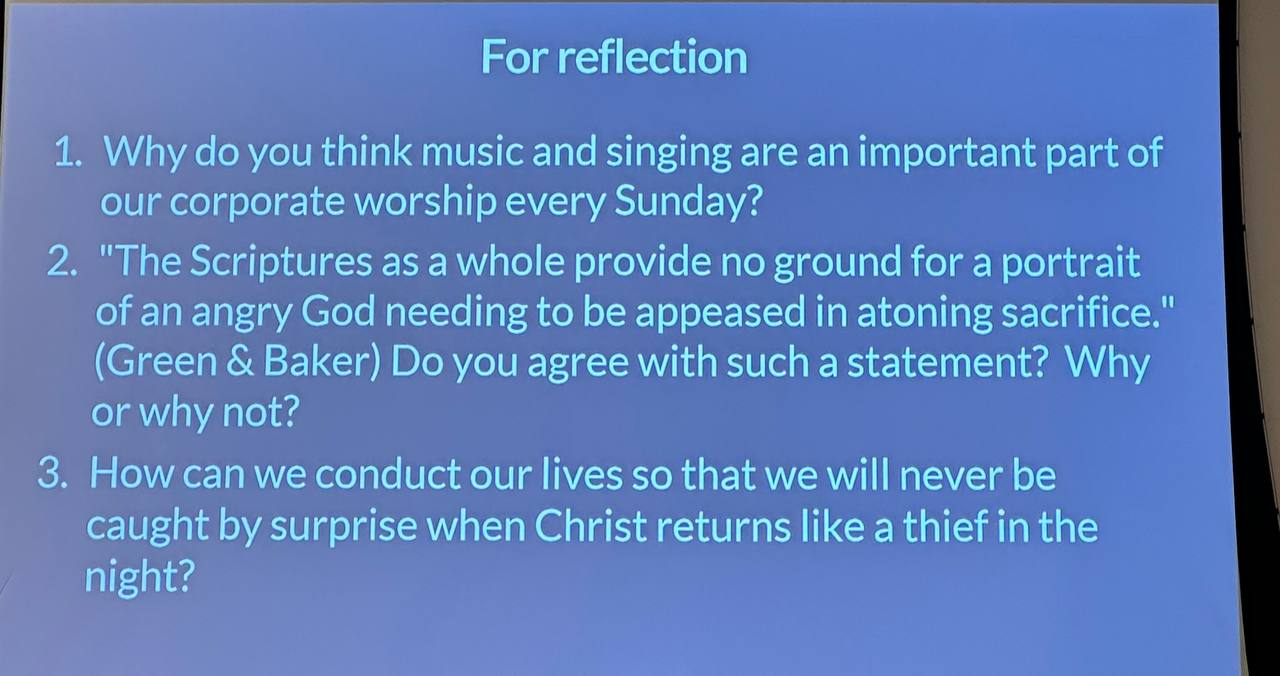
\includegraphics[width=0.8\textwidth, trim={0cm 0cm 0cm 0cm},clip]{Figures/marchSermon4Reflections.jpg}
  %   \includegraphics[width=0.8\textwidth, trim={0cm 0cm 0cm 0cm},clip]{example-image-a}
  %   \caption[]{Reflection questions for this sermon}
  %   \label{}
  % \end{figure}}
\end{itemize}